%!TEX root = problems.tex

%\printanswers

\begin{questions}


\question
Construct all (non-isomorphic) trees of heights from one to four, that have five vertices.~\cite{biggs02}. Note that there is one of height one, four of height two, three of height three, and one of height four.
\begin{solution}

\begin{center}
  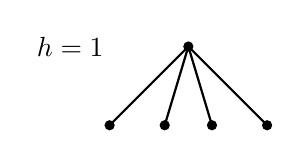
\begin{tikzpicture}
  \begin{scope}[every node/.style={thick,draw,circle,fill,scale=0.3}]
  \node (a) at (1,1) {};
  \node (b) at (0,0) {};
  \node (c) at (0.7,0) {};
  \node (d) at (1.3,0) {};
  \node (e) at (2,0) {};
  \end{scope}
  \begin{scope}[every edge/.style={draw=black,thick}]
  \path (a) edge (b);
  \path (a) edge (c);
  \path (a) edge (d);
  \path (a) edge (e);
  \end{scope}
  \node (l) at (-0.5,1) {$h = 1$};
  \end{tikzpicture}
\end{center}


\begin{center}
  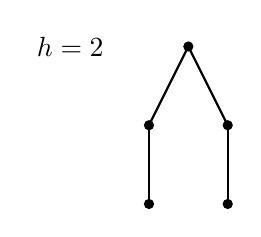
\begin{tikzpicture}
  \begin{scope}[every node/.style={thick,draw,circle,fill,scale=0.3}]
  \node (a) at (0.5,2) {};
  \node (b) at (0,1) {};
  \node (c) at (1,1) {};
  \node (d) at (0,0) {};
  \node (e) at (1,0) {};
  \end{scope}
  \begin{scope}[every edge/.style={draw=black,thick}]
  \path (a) edge (b);
  \path (a) edge (c);
  \path (b) edge (d);
  \path (c) edge (e);
  \end{scope}
  \node (l) at (-1,2) {$h = 2$};
  \end{tikzpicture}
  \hspace{0.4cm}
  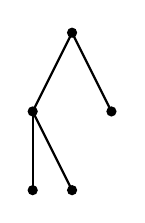
\begin{tikzpicture}
  \begin{scope}[every node/.style={thick,draw,circle,fill,scale=0.3}]
  \node (a) at (0.5,2) {};
  \node (b) at (0,1) {};
  \node (c) at (1,1) {};
  \node (d) at (0,0) {};
  \node (e) at (0.5,0) {};
  \end{scope}
  \begin{scope}[every edge/.style={draw=black,thick}]
  \path (a) edge (b);
  \path (a) edge (c);
  \path (b) edge (d);
  \path (b) edge (e);
  \end{scope}
  \end{tikzpicture}
  \hspace{0.4cm}
  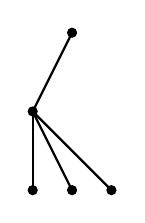
\begin{tikzpicture}
  \begin{scope}[every node/.style={thick,draw,circle,fill,scale=0.3}]
  \node (a) at (0.5,2) {};
  \node (b) at (0,1) {};
  \node (c) at (0,0) {};
  \node (d) at (0.5,0) {};
  \node (e) at (1,0) {};
  \end{scope}
  \begin{scope}[every edge/.style={draw=black,thick}]
  \path (a) edge (b);
  \path (b) edge (c);
  \path (b) edge (d);
  \path (b) edge (e);
  \end{scope}
  \end{tikzpicture}
  \hspace{0.4cm}
  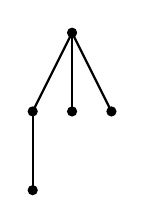
\begin{tikzpicture}
  \begin{scope}[every node/.style={thick,draw,circle,fill,scale=0.3}]
  \node (a) at (0.5,2) {};
  \node (b) at (0,1) {};
  \node (c) at (0.5,1) {};
  \node (d) at (1,1) {};
  \node (e) at (0,0) {};
  \end{scope}
  \begin{scope}[every edge/.style={draw=black,thick}]
  \path (a) edge (b);
  \path (a) edge (c);
  \path (a) edge (d);
  \path (b) edge (e);
  \end{scope}
  \end{tikzpicture}
\end{center}

\begin{center}
  \begin{tikzpicture}
  \begin{scope}[every node/.style={thick,draw,circle,fill,scale=0.3}]
  \node (a) at (0.5,3) {};
  \node (b) at (0,2) {};
  \node (c) at (1,2) {};
  \node (d) at (0,1) {};
  \node (e) at (0,0) {};
  \end{scope}
  \begin{scope}[every edge/.style={draw=black,thick}]
  \path (a) edge (b);
  \path (a) edge (c);
  \path (b) edge (d);
  \path (d) edge (e);
  \end{scope}
  \node (l) at (-1,3) {$h = 3$};
  \end{tikzpicture}
  \hspace{0.4cm}
  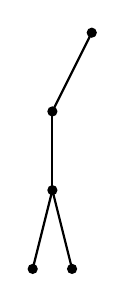
\begin{tikzpicture}
  \begin{scope}[every node/.style={thick,draw,circle,fill,scale=0.3}]
  \node (a) at (0.5,3) {};
  \node (b) at (0,2) {};
  \node (c) at (0,1) {};
  \node (d) at (-0.25,0) {};
  \node (e) at (0.25,0) {};
  \end{scope}
  \begin{scope}[every edge/.style={draw=black,thick}]
  \path (a) edge (b);
  \path (b) edge (c);
  \path (c) edge (d);
  \path (c) edge (e);
  \end{scope}
  \end{tikzpicture}
  \hspace{0.4cm}
  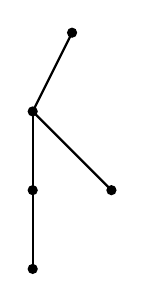
\begin{tikzpicture}
  \begin{scope}[every node/.style={thick,draw,circle,fill,scale=0.3}]
  \node (a) at (0.5,3) {};
  \node (b) at (0,2) {};
  \node (c) at (0,1) {};
  \node (d) at (1,1) {};
  \node (e) at (0,0) {};
  \end{scope}
  \begin{scope}[every edge/.style={draw=black,thick}]
  \path (a) edge (b);
  \path (b) edge (d);
  \path (b) edge (c);
  \path (c) edge (e);
  \end{scope}
  \end{tikzpicture}
\end{center}

\begin{center}
  \begin{tikzpicture}
  \begin{scope}[every node/.style={thick,draw,circle,fill,scale=0.3}]
  \node (a) at (0,4) {};
  \node (b) at (0,3) {};
  \node (c) at (0,2) {};
  \node (d) at (0,1) {};
  \node (e) at (0,0) {};
  \end{scope}
  \begin{scope}[every edge/.style={draw=black,thick}]
  \path (a) edge (b);
  \path (b) edge (c);
  \path (c) edge (d);
  \path (d) edge (e);
  \end{scope}
  \node (l) at (-1,3) {$h = 4$};
  \end{tikzpicture}
\end{center}

\end{solution}


\question
Construct two non-isomorphic rooted trees both having twelve vertices, six leaves, and height four~\cite{biggs02}.
\begin{solution}


\begin{center}
  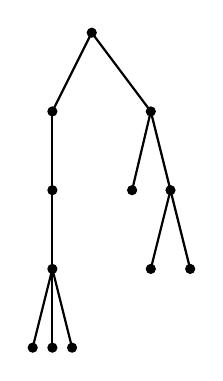
\begin{tikzpicture}
  \begin{scope}[every node/.style={thick,draw,circle,fill,scale=0.3}]
  \node (a) at (-0.5,4) {};
  \node (b) at (-1,3) {};
  \node (c) at (0.25,3) {};
  \node (d) at (-1,2) {};
  \node (e) at (0.0125,2) {};
  \node (f) at (0.5,2) {};
  \node (g) at (-1,1) {};
  \node (h) at (0.25,1) {};
  \node (i) at (0.75,1) {};
  \node (j) at (-1.25,0) {};
  \node (k) at (-1,0) {};
  \node (l) at (-0.75,0) {};
  \end{scope}
  \begin{scope}[every edge/.style={draw=black,thick}]
  \path (a) edge (b);
  \path (a) edge (c);
  \path (b) edge (d);
  \path (c) edge (e);
  \path (c) edge (f);
  \path (d) edge (g);
  \path (f) edge (h);
  \path (f) edge (i);
  \path (d) edge (g);
  \path (g) edge (j);
  \path (g) edge (k);
  \path (g) edge (l);
  \end{scope}
  \end{tikzpicture}
  \hspace{2cm}
  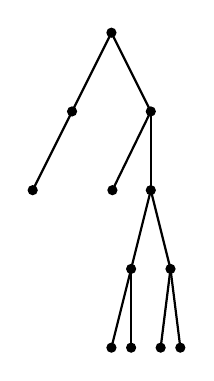
\begin{tikzpicture}
  \begin{scope}[every node/.style={thick,draw,circle,fill,scale=0.3}]
  \node (a) at (0,4) {};
  \node (b) at (-0.5,3) {};
  \node (c) at (0.5,3) {};
  \node (d) at (-1,2) {};
  \node (e) at (0.0125,2) {};
  \node (f) at (0.5,2) {};
  \node (g) at (0.25,1) {};
  \node (h) at (0.75,1) {};
  \node (i) at (0,0) {};
  \node (j) at (0.25,0) {};
  \node (k) at (0.625,0) {};
  \node (l) at (0.875,0) {};
  \end{scope}
  \begin{scope}[every edge/.style={draw=black,thick}]
  \path (a) edge (b);
  \path (a) edge (c);
  \path (b) edge (d);
  \path (c) edge (e);
  \path (c) edge (f);
  \path (f) edge (g);
  \path (f) edge (h);
  \path (g) edge (i);
  \path (g) edge (j);
  \path (h) edge (k);
  \path (h) edge (l);
  \end{scope}
  \end{tikzpicture}
\end{center}

\end{solution}

\question
Calculate the minimum height of a ternary rooted tree with ten leaves.
\begin{solution}


We have that $h \leq  \log_m l$.
Now, $\log_3 10 \approx 2.096$.
Since the minimum height must be a natural number, and this is a lower bound, we have that the minimum height is 3.
\end{solution}

\question
Draw a ternary decision tree of height at most two, representing the following problem.

Suppose you have access to the international prototype kilogram.
This is a weight, kept in France, which is the definition of the kilogram.
You are presented with four other weights which are supposed to each be exactly one kilogram.
However, you suspect that one of them is not a kilogram in weight but you can't tell which one it is.
You don't have access to a weighing scales, but you do have access to a balance.
This balance can be used to compare the weights of various objects and combinations of objects.~\cite{biggs02}
\begin{solution}
\begin{center}
  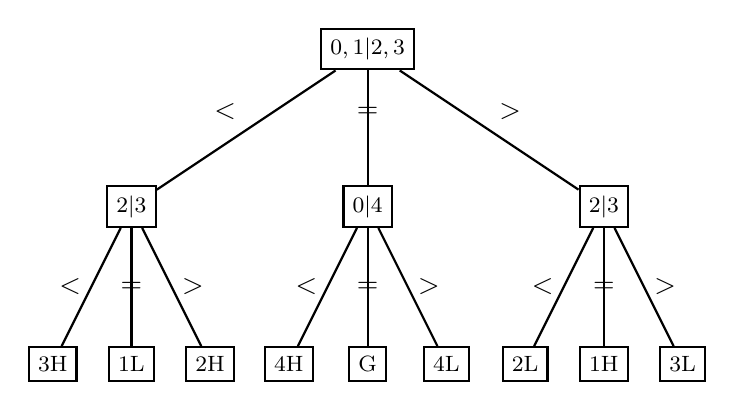
\begin{tikzpicture}
  \begin{scope}[every node/.style={thick,draw}]
  \node (a) at (0,4) {\footnotesize $0,1 | 2,3$};
  \node (b) at (-3,2) {\footnotesize $2 | 3$};
  \node (c) at (0,2) {\footnotesize $0 | 4$};
  \node (d) at (3,2) {\footnotesize $2 | 3$};
  \node (e) at (-4,0) {\footnotesize 3H};
  \node (f) at (-3,0) {\footnotesize 1L};
  \node (g) at (-2,0) {\footnotesize 2H};
  \node (h) at (-1,0) {\footnotesize 4H};
  \node (i) at (0,0) {\footnotesize G};
  \node (j) at (1,0) {\footnotesize 4L};
  \node (k) at (2,0) {\footnotesize 2L};
  \node (l) at (3,0) {\footnotesize 1H};
  \node (m) at (4,0) {\footnotesize 3L};
  \end{scope}
  \begin{scope}[every edge/.style={draw=black,thick}]
  \path (a) edge node[above left] {$<$}  (b);
  \path (a) edge node[above] {$=$}  (c);
  \path (a) edge node[above right] {$>$} (d);
  \path (b) edge node[left] {$<$}  (e);
  \path (b) edge node[] {$=$}  (f);
  \path (b) edge node[right] {$>$} (g);
  \path (c) edge node[left] {$<$}  (h);
  \path (c) edge node[] {$=$}  (i);
  \path (c) edge node[right] {$>$} (j);
  \path (d) edge node[left] {$<$}  (k);
  \path (d) edge node[] {$=$}  (l);
  \path (d) edge node[right] {$>$} (m);
  \end{scope}
  \end{tikzpicture}
\end{center}

\end{solution}

\question
Draw a decision tree for bubble sort with three elements.~\cite{biggs02}
\begin{solution}
\begin{center}
  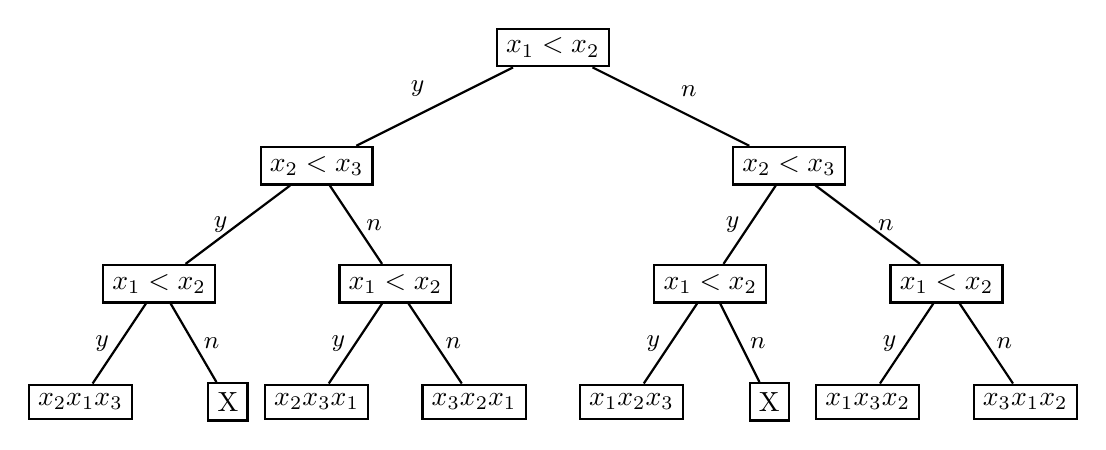
\begin{tikzpicture}
  \begin{scope}[every node/.style={thick,draw}]
  \node (a) at (4,6) {$x_1 < x_2$};
  \node (b) at (1,4.5) {$x_2 < x_3$};
  \node (c) at (7,4.5) {$x_2 < x_3$};
  \node (d) at (-1,3) {$x_1 < x_2$};
  \node (e) at (2,3) {$x_1 < x_2$};
  \node (f) at (6,3) {$x_1 < x_2$};
  \node (g) at (9,3) {$x_1 < x_2$};
  \node (h) at (-2,1.5) {$x_2 x_1 x_3$};
  \node (i) at (-0.125,1.5) {X};
  \node (j) at (1,1.5) {$x_2 x_3 x_1$};
  \node (k) at (3,1.5) {$x_3 x_2 x_1$};
  \node (l) at (5,1.5) {$x_1 x_2 x_3$};
  \node (m) at (6.75,1.5) {X};
  \node (n) at (8,1.5) {$x_1 x_3 x_2$};
  \node (o) at (10,1.5) {$x_3 x_1 x_2$};
  \end{scope}
  \begin{scope}[every edge/.style={draw=black,thick}]
  \path (a) edge node[above left] {\small $y$} (b);
  \path (a) edge node[above right] {\small $n$} (c);
  \path (b) edge node[left] {\small $y$} (d);
  \path (b) edge node[right] {\small $n$} (e);
  \path (c) edge node[left] {\small $y$} (f);
  \path (c) edge node[right] {\small $n$} (g);
  \path (d) edge node[left] {\small $y$} (h);
  \path (d) edge node[right] {\small $n$} (i);
  \path (e) edge node[left] {\small $y$} (j);
  \path (e) edge node[right] {\small $n$} (k);
  \path (f) edge node[left] {\small $y$} (l);
  \path (f) edge node[right] {\small $n$} (m);
  \path (g) edge node[left] {\small $y$} (n);
  \path (g) edge node[right] {\small $n$} (o);
  \end{scope}
  \end{tikzpicture}
\end{center}
\end{solution}



\question
What is the smallest possible height of the decision tree of an algorithm for sorting four objects using binary comparisons?~\cite{biggs02}
\begin{solution}

Number of outcomes (leaves) is $l = 4! = 24$.
Binary tree, so $m = 2$.
So minimum height is $log_2 24 \approx 4.58$.
Rounding up, gives smallest height as 5.
\end{solution}

\question
Calculate the minimum number of binary comparisons needed (in the worst case) when four objects are sorted~\cite{biggs02}.
\begin{parts}
  \part by bubble sort.
  \part by insertion (sequential method).
  \part by insertion (bisection method).
\end{parts}
\begin{solution}
\begin{parts}
\part $3 + 2 + 1 = 6$
\part $1 + 2 + 3 = 6$
\part $1 + 2 + 2 = 5$.
\end{parts}
\end{solution}

\end{questions}

\begin{thebibliography}{9}

\bibitem{biggs02}
  Norman Biggs,
  \emph{Discrete Mathematics},
  Oxford University Press,
  2nd edition,
  2002.
\end{thebibliography}
